{\bf BME154L - Spring 2012 - Exam \#2 Solutions}\hfill Name (Net ID):\underline{\hspace*{3.0in}}



\section{[50 points]}

\begin{center}
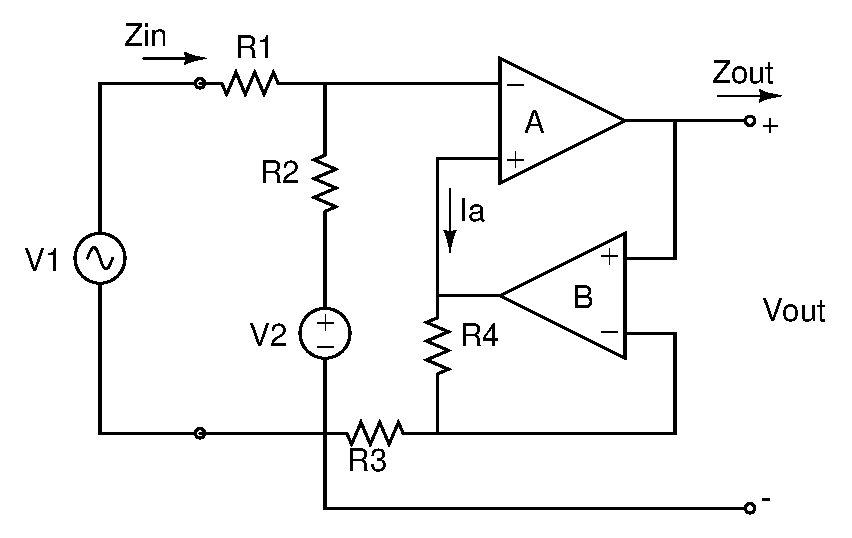
\includegraphics[width=0.75\linewidth]{comparator/comparator.eps}
\end{center}

All of the components in the circuit above should be considered ideal and have the following values:
\begin{itemize}
	\item Component Values: $R_1 = R_2 = R_3 = R_4 = 10$ k$\Omega$; $V_2$ = -1 V
	\item Rail voltages for op amp A: $\pm$ 2 V
	\item Rail voltages for op amp B: $\pm$ 12 V
\end{itemize}

\begin{enumerate}
	\item What is the input impedance ($Z_\textrm{in}$), as indicated on the circuit diagram (as ``seen'' by $V_1$). [5 points]
	\item Op amp A is configured with {\bf [ no / negative / positive ]} feedback. Why? [5 points, choose one answer]
	\item Op amp B is configured with {\bf [ no / negative / positive ]} feedback. Why? [5 points, choose one answer]
        \item Write an expression for $I_a$, as indicated on the circuit diagram. [5 points]
        \item What is the purpose of $V_2$ in this circuit? [5 points]
	\item Sketch $V_\textrm{out}$ for $V_1$ = -12:12 V.  Please be sure to indicate the overall function of this circuit and show your steps in solving for $V_\textrm{out}$ to maximize partial credit!! [15 points]
	\item Sketch $V_\textrm{out}$ for 2 cycles of $V_1$ = 12 $\cos(100t)$ V, starting at $t$ = 0. [5 points]
	\item What is the output impedance, $Z_\textrm{out}$, as indicated on the circuit diagram? [5 points]
\end{enumerate}
